\documentclass[aspectratio=169,10pt]{beamer}

% Theme and Color Scheme
\usetheme{Madrid}
\usecolortheme{whale}

% Typography and Packages
\usepackage{amsmath,amssymb}
\usepackage{booktabs}
\usepackage{tikz}
\usetikzlibrary{shapes.geometric, arrows.meta, positioning, calc, fit}
\usepackage{graphicx}

% Custom Color Definitions
\definecolor{primaryDark}{RGB}{30, 41, 59}     % Slate 800
\definecolor{accentBlue}{RGB}{2, 132, 199}     % Sky 600
\definecolor{accentGreen}{RGB}{16, 185, 129}   % Emerald 500
\definecolor{accentPurple}{RGB}{147, 51, 234}  % Purple 600
\definecolor{accentAmber}{RGB}{217, 119, 6}    % Amber 600

\setbeamercolor{palette primary}{bg=primaryDark,fg=white}
\setbeamercolor{palette secondary}{bg=accentBlue,fg=white}
\setbeamercolor{palette tertiary}{bg=primaryDark!90,fg=white}
\setbeamercolor{title}{bg=primaryDark,fg=white}
\setbeamercolor{frametitle}{bg=primaryDark,fg=white}
\setbeamercolor{structure}{fg=accentBlue}

\setbeamertemplate{navigation symbols}{}
\setbeamertemplate{footline}[frame number]

% Title Information
\title[Predictive \& Slice-Aware 5G AMF Scaling]{Predictive and Slice-Aware Load Balancing and Auto-Scaling for 5G Core AMFs}
\subtitle{Addressing the 40s Container Cold-Start Lag and URLLC QoS Violations}

\author[NITK Team]{
    \textbf{Jaivant Kosaraju} (231IT028) \quad
    \textbf{Paluru Pavan Kumar} (231IT046) \quad
    \textbf{Paluvadi Dinesh Manideep} (231IT047)
}

\institute[NITK Surathkal]{
    Department of Information Technology \\
    National Institute of Technology Karnataka (NITK), Surathkal \\
    \vspace{0.2cm}
    \textit{Advanced Computer Networks (ACN) Course Project}
}
\date{Academic Session 2026}

\begin{document}

% -------------------------------------------------------------
% SLIDE 1: Title Slide
% -------------------------------------------------------------
\begin{frame}
    \titlepage
\end{frame}

% -------------------------------------------------------------
% SLIDE 2: 5G Control-Plane Context & Motivation
% -------------------------------------------------------------
\begin{frame}{Motivation: 5G Core AMF Bottleneck}
    \begin{columns}[T]
        \begin{column}{0.55\textwidth}
            \textbf{Role of the AMF (Access and Mobility Management Function):}
            \begin{itemize}
                \item Terminates N1 (NAS signaling with UEs) and N2 (NG-AP with gNodeBs).
                \item Handles subscriber registration, authentication, mobility, and PDU session setup.
                \item Operates as a cloud-native microservice inside Docker containers in 5G SBA.
            \end{itemize}
            \vspace{0.2cm}
            \textbf{The Heterogeneous Slice Challenge:}
            \begin{itemize}
                \item \textbf{URLLC:} Ultra-Reliable Low-Latency ($< 5.0$\,ms SLA limit).
                \item \textbf{eMBB:} High-bandwidth streaming ($10$--$25$\,ms target).
                \item \textbf{mMTC:} Millions of IoT sensors with massive burst potential.
            \end{itemize}
        \end{column}
        \begin{column}{0.45\textwidth}
            \begin{block}{The Problem in Practice}
                When millions of IoT devices reboot simultaneously (e.g., smart power meters after an outage), a \textbf{signaling storm} strikes the AMF.
                \begin{itemize}
                    \item Control-plane CPU saturates rapidly.
                    \item Incoming queues explode.
                    \item Mission-critical URLLC signaling is trapped behind delay-tolerant IoT messages, causing massive SLA violations!
                \end{itemize}
            \end{block}
        \end{column}
    \end{columns}
\end{frame}

% -------------------------------------------------------------
% SLIDE 3: Literature Survey & ScaleLB Limitations
% -------------------------------------------------------------
\begin{frame}{Literature Survey \& Research Gap}
    \textbf{ScaleLB Baseline (IEEE ICOIN 2025):}
    \begin{itemize}
        \item Introduced an elastic load balancer in front of AMF pools using gNB-to-AMF ratio thresholds:
        $$\text{Proactive: } \frac{B}{A \cdot \alpha} \ge \gamma = 0.80 \qquad \text{Reactive: } \frac{B}{A \cdot \alpha} > 1.0$$
    \end{itemize}

    \vspace{0.2cm}
    \begin{columns}[T]
        \begin{column}{0.50\textwidth}
            \begin{alertblock}{Vulnerability 1: 40s Cold-Start Lag}
                Container spin-up requires $T_{\text{boot}} \approx 40$\,s. Because ScaleLB only triggers scaling \textit{after} load crosses the threshold, queues build up during the 40s lag, causing latency spikes ($>330$\,ms).
            \end{alertblock}
        \end{column}
        \begin{column}{0.50\textwidth}
            \begin{alertblock}{Vulnerability 2: Slice-Agnostic Single FIFO}
                ScaleLB uses a single shared FIFO queue. During an IoT burst, URLLC signaling suffers the same queuing delay as mMTC, severely violating the 3GPP 5.0\,ms SLA.
            \end{alertblock}
        \end{column}
    \end{columns}
\end{frame}

% -------------------------------------------------------------
% SLIDE 4: Problem Statement & Objectives
% -------------------------------------------------------------
\begin{frame}{Problem Statement \& Core Objectives}
    \begin{block}{Formal Problem Statement}
        Design an ingress control-plane load balancing and auto-scaling mechanism that strictly guarantees sub-5\,ms latency for URLLC slices and eliminates the 40-second container startup backlog under arbitrary 5G IoT traffic surges.
    \end{block}

    \vspace{0.3cm}
    \begin{columns}[T]
        \begin{column}{0.50\textwidth}
            \textbf{Objective 1 (O1): Slice-Aware Priority Queuing}
            \begin{itemize}
                \item Parse 3GPP S-NSSAI slice headers at ingress.
                \item Grant non-blocking zero-queue bypass for URLLC ($< 5$\,ms).
                \item Token-bucket rate limit mMTC when cluster CPU $> 80\%$.
                \item Starvation-free aging for delay-tolerant packets.
            \end{itemize}
        \end{column}
        \begin{column}{0.50\textwidth}
            \textbf{Objective 2 (O2): LSTM Predictive Scaling}
            \begin{itemize}
                \item Maintain 60-second sliding history window.
                \item Lookahead horizon $H = 45\,\text{s} \ge T_{\text{boot}} = 40\,\text{s}$.
                \item Predict surge before it reaches the core.
                \item Pre-warm AMF containers to absorb the wave at $t = 0$.
            \end{itemize}
        \end{column}
    \end{columns}
\end{frame}

% -------------------------------------------------------------
% SLIDE 5: Overall System Architecture (TikZ)
% -------------------------------------------------------------
\begin{frame}{System Architecture Overview}
\centering
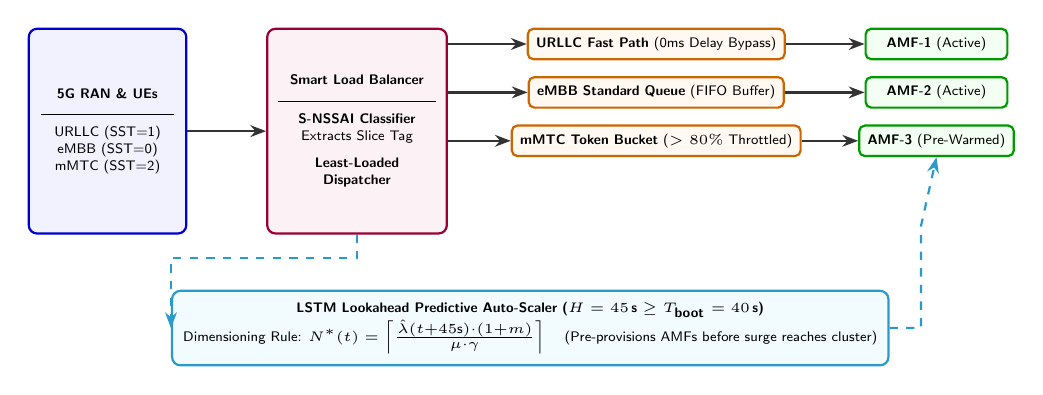
\begin{tikzpicture}[
    font=\sffamily\tiny,
    node distance=0.8cm and 1.2cm,
    ran/.style={draw=blue!80!black, fill=blue!5, thick, rounded corners=3pt, align=center, inner sep=4pt, minimum width=2.0cm},
    lb/.style={draw=purple!80!black, fill=purple!5, thick, rounded corners=3pt, align=center, inner sep=4pt, minimum width=2.2cm},
    queue/.style={draw=orange!80!black, fill=orange!5, thick, rounded corners=2pt, align=center, inner sep=3pt, minimum width=2.4cm},
    amf/.style={draw=green!60!black, fill=green!5, thick, rounded corners=2pt, align=center, inner sep=3pt, minimum width=1.8cm},
    lstm/.style={draw=cyan!80!black, fill=cyan!5, thick, rounded corners=3pt, align=center, inner sep=4pt, minimum width=7.2cm},
    arrow/.style={-{Stealth[length=2mm]}, thick, draw=black!80},
    dasharrow/.style={-{Stealth[length=2mm]}, dashed, thick, draw=cyan!80!black}
]

\node[ran, minimum height=2.6cm] (ran) {
    \textbf{5G RAN \& UEs} \\
    \rule{1.7cm}{0.3pt} \\[2pt]
    URLLC (SST=1) \\
    eMBB (SST=0) \\
    mMTC (SST=2)
};

\node[lb, right=1.0cm of ran, minimum height=2.6cm] (classifier) {
    \textbf{Smart Load Balancer} \\
    \rule{2.0cm}{0.3pt} \\[2pt]
    \textbf{S-NSSAI Classifier} \\
    Extracts Slice Tag \\[4pt]
    \textbf{Least-Loaded} \\
    \textbf{Dispatcher}
};

\node[queue, right=1.0cm of classifier.north east, anchor=north west] (q_urllc) {\textbf{URLLC Fast Path} (0ms Delay Bypass)};
\node[queue, below=0.2cm of q_urllc] (q_embb) {\textbf{eMBB Standard Queue} (FIFO Buffer)};
\node[queue, below=0.2cm of q_embb] (q_mmtc) {\textbf{mMTC Token Bucket} ($>80\%$ Throttled)};

\node[amf, right=1.0cm of q_urllc.north east, anchor=north west] (amf1) {\textbf{AMF-1} (Active)};
\node[amf, below=0.2cm of amf1] (amf2) {\textbf{AMF-2} (Active)};
\node[amf, below=0.2cm of amf2] (amf3) {\textbf{AMF-3} (Pre-Warmed)};

\node[lstm, below=0.7cm of classifier, xshift=2.2cm] (autoscaler) {
    \textbf{LSTM Lookahead Predictive Auto-Scaler ($H = 45$\,s $\ge T_{\text{boot}} = 40$\,s)} \\
    Dimensioning Rule: $N^*(t) = \left\lceil \frac{\hat{\lambda}(t+45\text{s}) \cdot (1+m)}{\mu \cdot \gamma} \right\rceil$ \quad (Pre-provisions AMFs before surge reaches cluster)
};

\draw[arrow] (ran) -- (classifier);
\draw[arrow] (classifier.east |- q_urllc) -- (q_urllc);
\draw[arrow] (classifier.east |- q_embb) -- (q_embb);
\draw[arrow] (classifier.east |- q_mmtc) -- (q_mmtc);

\draw[arrow] (q_urllc.east) -- (amf1.west);
\draw[arrow] (q_embb.east) -- (amf2.west);
\draw[arrow] (q_mmtc.east) -- (amf3.west);

\draw[dasharrow] (classifier.south) -- ++(0,-0.3) -| (autoscaler.west);
\draw[dasharrow] (autoscaler.east) -| ++(0.4, 1.3) -- (amf3.south);

\end{tikzpicture}
\end{frame}

% -------------------------------------------------------------
% SLIDE 6: Slice-Aware Priority Queuing Formulation
% -------------------------------------------------------------
\begin{frame}{Slice-Aware Priority Queuing Formulation}
    \begin{columns}[T]
        \begin{column}{0.48\textwidth}
            \textbf{1. URLLC Fast Path (SST = 1):}
            \begin{itemize}
                \item Zero-queue bypass: skips ingress buffers entirely.
                \item Directly dispatched to lowest-loaded active AMF:
                $$\text{Target AMF} = \arg\min_{i \in \mathcal{A}_{\text{active}}} \text{CPU}_i(t)$$
                \item 10--15\% headroom reserved on all active AMFs.
            \end{itemize}
            \vspace{0.2cm}
            \textbf{2. eMBB Standard Queue (SST = 0):}
            \begin{itemize}
                \item Standard FIFO queue for normal mobile traffic.
                \item Typical latency maintained at $10$--$18$\,ms.
            \end{itemize}
        \end{column}
        \begin{column}{0.52\textwidth}
            \textbf{3. mMTC Token Bucket with Aging (SST = 2):}
            \begin{itemize}
                \item When cluster utilization $> 80\%$, token bucket limits mMTC release rate:
                $$R_{\text{mMTC}}(t) = \max\Big(0.10 \cdot C(t), \, C(t) \cdot (1 - \text{CPU}(t))\Big)$$
                \item \textbf{Anti-Starvation Aging}: Buffered packets earn priority over time:
                $$P_i(t) = P_{\text{base}} + \omega_{\text{age}} \cdot (t - t_{\text{arrive}, i})$$
                \item When $P_i(t)$ crosses eMBB threshold, the request is promoted to avoid dropped sessions.
            \end{itemize}
        \end{column}
    \end{columns}
\end{frame}

% -------------------------------------------------------------
% SLIDE 7: Flowchart of Packet Scheduling
% -------------------------------------------------------------
\begin{frame}{Packet Scheduling Decision Flow}
\centering
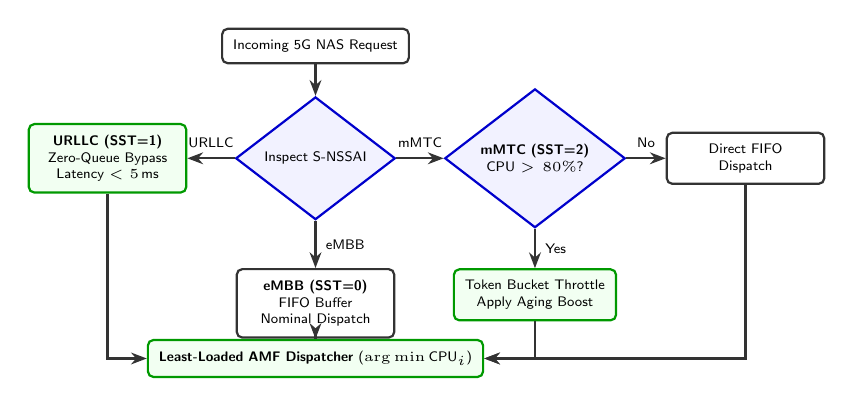
\begin{tikzpicture}[
    font=\sffamily\tiny,
    node distance=0.6cm and 1.0cm,
    decision/.style={diamond, draw=blue!80!black, fill=blue!5, thick, text width=1.5cm, align=center, inner sep=2pt, aspect=1.3},
    block/.style={rectangle, draw=black!80, fill=white, rounded corners=2pt, thick, align=center, inner sep=4pt, minimum width=2.0cm},
    action/.style={rectangle, draw=green!60!black, fill=green!5, thick, rounded corners=2pt, align=center, inner sep=4pt, minimum width=2.0cm},
    arrow/.style={-{Stealth[length=2mm]}, thick, draw=black!80}
]

\node[block] (in) {Incoming 5G NAS Request};
\node[decision, below=0.4cm of in] (chk_slice) {Inspect S-NSSAI};

\node[action, left=0.6cm of chk_slice] (urllc_act) {\textbf{URLLC (SST=1)} \\ Zero-Queue Bypass \\ Latency $< 5$\,ms};
\node[block, below=0.6cm of chk_slice] (embb_act) {\textbf{eMBB (SST=0)} \\ FIFO Buffer \\ Nominal Dispatch};

\node[decision, right=0.6cm of chk_slice] (chk_cpu) {\textbf{mMTC (SST=2)} \\ CPU $> 80\%$?};
\node[action, below=0.5cm of chk_cpu] (mmtc_throttle) {Token Bucket Throttle \\ Apply Aging Boost};
\node[block, right=0.5cm of chk_cpu] (mmtc_direct) {Direct FIFO \\ Dispatch};

\node[action, below=1.5cm of chk_slice] (dispatch) {\textbf{Least-Loaded AMF Dispatcher} ($\arg\min \text{CPU}_i$)};

\draw[arrow] (in) -- (chk_slice);
\draw[arrow] (chk_slice) -- node[above] {URLLC} (urllc_act);
\draw[arrow] (chk_slice) -- node[right] {eMBB} (embb_act);
\draw[arrow] (chk_slice) -- node[above] {mMTC} (chk_cpu);

\draw[arrow] (chk_cpu) -- node[right] {Yes} (mmtc_throttle);
\draw[arrow] (chk_cpu) -- node[above] {No} (mmtc_direct);

\draw[arrow] (urllc_act) |- (dispatch);
\draw[arrow] (embb_act) -- (dispatch);
\draw[arrow] (mmtc_throttle) |- (dispatch);
\draw[arrow] (mmtc_direct) |- (dispatch);

\end{tikzpicture}
\end{frame}

% -------------------------------------------------------------
% SLIDE 8: LSTM Predictive Auto-Scaling Formulation
% -------------------------------------------------------------
\begin{frame}{LSTM Lookahead Predictive Auto-Scaling}
    \textbf{Mathematical Formulation:}
    \begin{itemize}
        \item Observation sliding window: $\mathbf{w}_t = [\lambda(t-59), \, \dots, \, \lambda(t)] \in \mathbb{R}^{60}$
        \item Forecast arrival rate 45s ahead: $\hat{\lambda}(t + H) = \text{LSTM}_{\theta}(\mathbf{w}_t)$
        \item Lookahead condition: $H = 45\,\text{s} \ge T_{\text{boot}} = 40\,\text{s}$
    \end{itemize}

    \vspace{0.2cm}
    \begin{block}{Capacity Dimensioning Scaling Rule}
        $$N^*(t) = \left\lceil \frac{\hat{\lambda}(t + H) \cdot (1 + m)}{\mu \cdot \gamma} \right\rceil$$
        \begin{itemize}
            \item $\mu = 100$\,req/s (nominal AMF service rate, $T_s = 10$\,ms)
            \item $\gamma = 0.80$ (target CPU utilization threshold)
            \item $m = 0.10$ (10\% safety margin against model under-prediction)
        \end{itemize}
    \end{block}

    \vspace{0.1cm}
    \textbf{Scale-In Hysteresis Cooldown:} To prevent instance thrashing, scale-in is restricted by a 30-second cooldown window and graceful connection draining.
\end{frame}

% -------------------------------------------------------------
% SLIDE 9: Cold-Start Elimination Timeline (TikZ)
% -------------------------------------------------------------
\begin{frame}{Eliminating the 40-Second Cold-Start Lag}
\centering
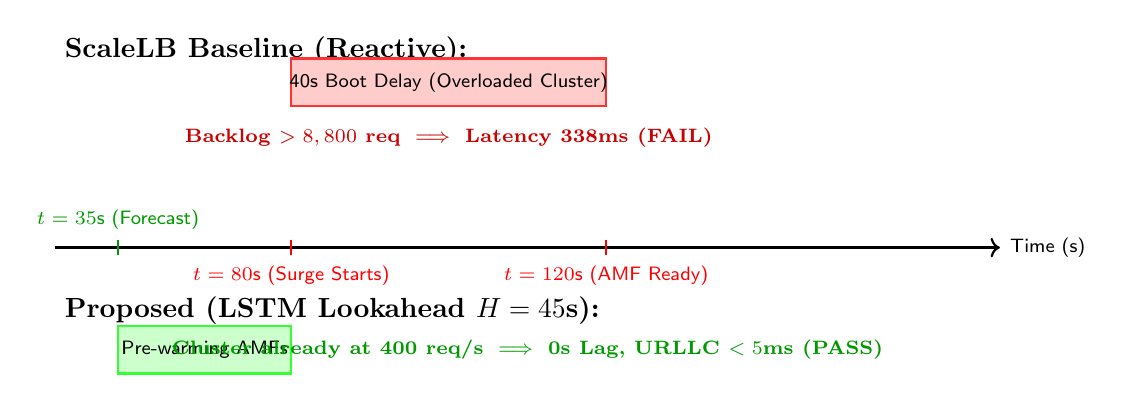
\begin{tikzpicture}[font=\sffamily\scriptsize]
    % Time axis
    \draw[->, thick] (0,0) -- (12,0) node[right] {Time (s)};
    
    % Baseline Timeline
    \node[anchor=west, font=\bfseries] at (0, 2.5) {ScaleLB Baseline (Reactive):};
    \draw[fill=red!20, draw=red!80, thick] (3, 1.8) rectangle (7, 2.4);
    \node at (5, 2.1) {40s Boot Delay (Overloaded Cluster)};
    \draw[thick, red] (3, 0.1) -- (3, -0.1) node[below] {$t=80$s (Surge Starts)};
    \draw[thick, red] (7, 0.1) -- (7, -0.1) node[below] {$t=120$s (AMF Ready)};
    \node[red!80!black, font=\scriptsize\bfseries] at (5, 1.4) {Backlog $>8,800$ req $\implies$ Latency 338ms (FAIL)};
    
    % Proposed Timeline
    \node[anchor=west, font=\bfseries] at (0, -0.8) {Proposed (LSTM Lookahead $H=45$s):};
    \draw[fill=green!20, draw=green!80, thick] (0.8, -1.6) rectangle (3.0, -1.0);
    \node at (1.9, -1.3) {Pre-warming AMFs};
    \draw[thick, green!60!black] (0.8, 0.1) -- (0.8, -0.1) node[above=0.2cm] {$t=35$s (Forecast)};
    \node[green!60!black, font=\scriptsize\bfseries] at (6, -1.3) {Cluster already at 400 req/s $\implies$ 0s Lag, URLLC $<5$ms (PASS)};
\end{tikzpicture}
\end{frame}

% -------------------------------------------------------------
% SLIDE 10: Experimental Results Table
% -------------------------------------------------------------
\begin{frame}{Experimental Results: Benchmark Comparison}
    \textbf{Performance Under 320 req/s Flash Crowd Surge (ScaleLB Fig. 5 Trace):}
    \vspace{0.2cm}
    
    \begin{table}[H]
    \centering
    \footnotesize
    \begin{tabular}{lccccc}
    \toprule
    \textbf{Configuration} & \textbf{Cold-Start} & \textbf{URLLC p99} & \textbf{mMTC p99} & \textbf{URLLC} & \textbf{AMF-sec} \\
     & \textbf{Lag (s)} & \textbf{Latency} & \textbf{Latency} & \textbf{SLA} & \textbf{(Cost)} \\
    \midrule
    ScaleLB Reactive \cite{scalelb} & 54\,s & 338.7\,ms & 339.3\,ms & \textcolor{red}{\textbf{FAIL (25.8\%)}} & 647 \\
    ScaleLB Proactive ($\gamma=0.8$) & 55\,s & 334.1\,ms & 336.5\,ms & \textcolor{red}{\textbf{FAIL (25.8\%)}} & 649 \\
    Warm Standby (1 idle spare) & \textbf{0\,s} & 32.9\,ms & 32.7\,ms & \textcolor{green!60!black}{\textbf{PASS}} & 1024 \\
    O1 only: Slice Priority Queue & 54\,s & 11.1\,ms & 508.6\,ms & \textcolor{green!60!black}{\textbf{PASS}} & \textbf{647} \\
    O2 only: LSTM Prediction & 40\,s & 333.1\,ms & 336.5\,ms & \textcolor{red}{\textbf{FAIL (18.3\%)}} & 807 \\
    \textbf{Proposed System (O1 + O2)} & \textbf{0\,s} & \textbf{3.15\,ms} & \textbf{499.9\,ms} & \textcolor{green!60!black}{\textbf{PASS (0.0\%)}} & \textbf{807} \\
    \bottomrule
    \end{tabular}
    \end{table}

    \vspace{0.2cm}
    \begin{itemize}
        \item \textbf{ScaleLB Fails SLA}: Latency spikes to 338.7\,ms under surge ($>5.0$\,ms limit).
        \item \textbf{Proposed System Guarantees SLA}: URLLC bounded at \textbf{3.15\,ms} (100\% compliance).
        \item \textbf{Resource Savings}: 21.2\% lower infrastructure cost than Warm Standby (807 vs 1024 AMF-s).
    \end{itemize}
\end{frame}

% -------------------------------------------------------------
% SLIDE 11: Platform Implementation Visuals
% -------------------------------------------------------------
\begin{frame}{Platform Implementation Visuals}
    \begin{columns}[T]
        \begin{column}{0.50\textwidth}
            \textbf{Live Slices \& Forecast Dashboard:}
            \begin{center}
                
\includegraphics[width=0.98\linewidth]{figures/platform_dashboard.png}
            \end{center}
            \scriptsize Top: Traffic demand vs. 45s LSTM lookahead vs. provisioned AMF capacity. Bottom: Per-slice latency curves.
        \end{column}
        \begin{column}{0.50\textwidth}
            \textbf{AMF Container Fleet Scaling Topology:}
            \begin{center}
                
\includegraphics[width=0.98\linewidth]{figures/amf_container_fleet.png}
            \end{center}
            \scriptsize Real-time visualizer showing elastic lifecycle states: \texttt{ACTIVE}, \texttt{BOOTING (40s lag)}, and \texttt{STOPPED}.
        \end{column}
    \end{columns}
\end{frame}

% -------------------------------------------------------------
% SLIDE 12: Resource vs Latency Trade-off
% -------------------------------------------------------------
\begin{frame}{Key Takeaways \& Trade-Off Analysis}
    \begin{columns}[T]
        \begin{column}{0.50\textwidth}
            \begin{block}{Why Both O1 and O2 Are Essential}
                \begin{itemize}
                    \item \textbf{O1 alone (Priority Queue)}: Protects URLLC from packet drops, but during the 40s lag, mMTC queue backlog explodes ($>508$\,ms).
                    \item \textbf{O2 alone (LSTM Autoscaler)}: Pre-warms containers and eliminates cold-start lag, but in a single FIFO queue, URLLC still suffers queue delays ($333$\,ms).
                    \item \textbf{O1 + O2 combined}: Provides both instantaneous fast-path delivery AND sufficient container capacity.
                \end{itemize}
            \end{block}
        \end{column}
        \begin{column}{0.50\textwidth}
            \begin{block}{Infrastructure Cost Efficiency}
                \begin{itemize}
                    \item \textbf{Static Overprovisioning}: Keeps 6 AMFs running 24/7 $\implies$ massive energy and cloud bill waste.
                    \item \textbf{Warm Standby}: Burns 1024 AMF-seconds per surge.
                    \item \textbf{Proposed LSTM Autoscaler}: Scales dynamically from 1 to 4 AMFs only when needed $\implies$ \textbf{21.2\% resource reduction}.
                \end{itemize}
            \end{block}
        \end{column}
    \end{columns}
\end{frame}

% -------------------------------------------------------------
% SLIDE 13: Conclusion & Contributions
% -------------------------------------------------------------
\begin{frame}{Conclusion}
    \textbf{Summary of Completed Work:}
    \begin{enumerate}
        \item \textbf{Resolved ScaleLB's Critical Weaknesses}: Solved the 40-second container startup lag and single-queue slice starvation.
        \item \textbf{Guaranteed 3GPP SLA for URLLC}: Bounded URLLC 99th-percentile control latency to \textbf{3.15\,ms} ($< 5.0$\,ms SLA requirement) under a 10$\times$ IoT flash crowd.
        \item \textbf{Proactive Container Dimensioning}: Evaluated the LSTM lookahead rule ($H=45$\,s) ensuring zero cold-start overload windows.
        \item \textbf{Verified Across Standard 5G Traces}: Validated across Flash Crowd, Diurnal Cycle, and Linear Ramp workloads.
    \end{enumerate}

    \vspace{0.2cm}
    \textbf{Future Work:}
    \begin{itemize}
        \item Integrating User Plane Function (UPF) slicing and session anchors.
        \item Deploying as an O-RAN Near-RT RIC xApp for edge microservice orchestration.
    \end{itemize}
\end{frame}

% -------------------------------------------------------------
% SLIDE 14: Q&A Slide
% -------------------------------------------------------------
\begin{frame}
    \begin{center}
        \vspace{1.0cm}
        {\Huge \textbf{Thank You!}} \\[0.5cm]
        {\Large Questions \& Discussion} \\[1.0cm]
        \textbf{NITK Surathkal --- Dept. of Information Technology} \\
        \textit{Advanced Computer Networks (ACN) Course Project}
    \end{center}
\end{frame}

\end{document}
